% CaelumFusion VGA Render-Control Unified Implementation
% Source-backed consolidation of the attached VGA control-map drafts, the
% system report, and the active RTL implementation.

\documentclass[11pt,letterpaper]{article}

\usepackage[margin=0.72in]{geometry}
\usepackage[T1]{fontenc}
\usepackage[utf8]{inputenc}
\usepackage{amsmath}
\usepackage{amssymb}
\usepackage{array}
\usepackage{booktabs}
\usepackage{longtable}
\usepackage{tabularx}
\usepackage{enumitem}
\usepackage[dvipsnames]{xcolor}
\usepackage{graphicx}
\usepackage{float}
\usepackage{tikz}
\usetikzlibrary{arrows.meta,positioning,calc,fit,backgrounds}
\usepackage{listings}
\usepackage[hidelinks]{hyperref}

\setlength{\parindent}{0pt}
\setlength{\parskip}{5pt}
\renewcommand{\arraystretch}{1.18}
\emergencystretch=3em
\setlist[itemize]{leftmargin=1.35em,itemsep=2pt,topsep=3pt}
\setlist[enumerate]{leftmargin=1.55em,itemsep=2pt,topsep=3pt}

\newcolumntype{Y}{>{\raggedright\arraybackslash}X}
\newcolumntype{L}[1]{>{\raggedright\arraybackslash}p{#1}}
\newcommand{\sig}[1]{\texttt{\detokenize{#1}}}
\newcommand{\file}[1]{\texttt{\detokenize{#1}}}
\newcommand{\param}[1]{\texttt{\detokenize{#1}}}
\newcommand{\view}[1]{\texttt{\detokenize{#1}}}
\newcommand{\bits}[1]{\texttt{\detokenize{#1}}}
\newcommand{\logiczero}{\texttt{1'b0}}
\newcommand{\logicone}{\texttt{1'b1}}

\definecolor{cfblue}{RGB}{20,74,123}
\definecolor{cfgreen}{RGB}{21,105,72}
\definecolor{cfamber}{RGB}{146,91,17}
\definecolor{cfpurple}{RGB}{82,61,130}
\definecolor{cfred}{RGB}{154,54,50}
\definecolor{cfgray}{RGB}{244,246,249}
\definecolor{cfline}{RGB}{60,68,76}

\tikzset{
  cfBlock/.style={draw=cfline, rounded corners=2pt, very thick, fill=cfgray,
                  align=center, minimum height=0.82cm, text width=3.0cm,
                  font=\small},
  cfSmall/.style={draw=cfline, rounded corners=2pt, thick, fill=white,
                  align=center, minimum height=0.62cm, text width=2.45cm,
                  font=\scriptsize},
  cfState/.style={draw=cfline, rounded corners=2pt, thick, fill=#1!12,
                  align=center, minimum height=0.78cm, text width=2.35cm,
                  font=\scriptsize},
  cfLayer/.style={draw=cfline, rounded corners=2pt, thick, fill=#1!12,
                  align=center, minimum height=0.54cm, text width=10.6cm,
                  font=\scriptsize},
  cfArrow/.style={-{Stealth[length=2.6mm]}, very thick, draw=cfline},
  cfCtrl/.style={-{Stealth[length=2.3mm]}, thick, draw=cfamber},
  cfDashed/.style={-{Stealth[length=2.3mm]}, thick, dashed, draw=cfline},
  screen/.style={draw=cfline, very thick, fill=white},
  screenRect/.style={draw=cfline, rounded corners=1pt, thick, align=center,
                     font=\tiny}
}

\lstdefinelanguage{Verilog}{
  morekeywords={module,endmodule,input,output,wire,reg,parameter,localparam,
    assign,always,begin,end,if,else,case,endcase,function,endfunction,
    generate,endgenerate,for,integer},
  sensitive=true,
  morecomment=[l]{//},
  morecomment=[s]{/*}{*/},
  morestring=[b]"
}

\lstset{
  language=Verilog,
  basicstyle=\ttfamily\scriptsize,
  keywordstyle=\color{cfblue}\bfseries,
  commentstyle=\color{cfgreen},
  columns=fullflexible,
  keepspaces=true,
  breaklines=true,
  frame=single,
  framerule=0.25pt,
  numbers=left,
  numberstyle=\tiny\color{gray},
  xleftmargin=1.2em,
  framexleftmargin=1.0em
}

\title{\textbf{CaelumFusion VGA Render-Control Unified Implementation}\\
\large Consolidated comparison, final RTL boundary, and migration notes}
\author{CaelumFusion Flight Control System}
\date{Source snapshot reviewed on 2026-07-06}

\begin{document}
\maketitle

\begin{abstract}
This document reduces the supplied VGA rendering control-map drafts, the Phase 6
draft variants, the broader flight-control system report, and the live RTL into
one source-backed implementation reference.  The unified implementation is the
active \file{caelumfusion_vga_render_control.v} boundary instantiated by
\file{caelumfusion_top_vga.v}.  It preserves the primary flight HUD, self-test
HUD stimulus, optional in-HUD sensor diagnostic page, optional full-screen
compass/MAG truth page, switch-encoded direct view selection, deterministic
render-layer priority, and SYS-to-PIX timing contracts.
\end{abstract}

\tableofcontents
\newpage

\section{Source Basis}

The attached material falls into four useful source classes.  The table below
records what was preserved from each source and how conflicts were resolved.

\begin{longtable}{L{0.14\linewidth} L{0.25\linewidth} L{0.31\linewidth} L{0.20\linewidth}}
\caption{Source reconciliation for the unified implementation.}
\label{tab:source-reconciliation}\\
\toprule
\textbf{Source} & \textbf{Role} & \textbf{Preserved information} & \textbf{Resolution} \\
\midrule
\endfirsthead
\toprule
\textbf{Source} & \textbf{Role} & \textbf{Preserved information} & \textbf{Resolution} \\
\midrule
\endhead
Control Map A &
Compact VGA-only control map and rendered PDF. &
Board-facing VGA contract, button/switch map, final output function, view
priority, layer stack, compact screen-layout diagrams, debug-view use cases,
and known rendering limitations. &
Kept as the concise operator/control perspective. \\
Phase 6 Map B &
Detailed VGA render-control draft variants. &
Module responsibilities, wrapper parameter map, legal view state table, legacy
hold priority, semantic visualization bundle, CDC and frame-stability contract,
truth/evidence boundaries, and verification gates. &
Kept as the detailed design contract, with live defaults refreshed from RTL. \\
System Report C &
Whole-system design review artifact. &
Requirements traceability, sensor protocol contracts, module hierarchy,
clock/reset strategy, WaveForms/MATLAB evidence chain, and system-level risk
register. &
Kept only where it constrains the VGA integration boundary. \\
Live RTL D &
Current project source tree. &
\file{caelumfusion_vga_render_control.v},
\file{caelumfusion_top_vga.v}, \file{flight_viz_suite_top.v},
\file{flight_visualizer_pix.v}, \file{flight_vga_page_mux_pix.v},
\file{planar_compass_truth_page_vga.v}, XDC mappings, and the focused
render-control testbench. &
Live RTL wins when drafts disagree. \\
\bottomrule
\end{longtable}

\section{Comparison Table}

For implementation purposes, the old functional split is best treated as two
rendering modules plus top-level control glue:
\begin{itemize}
  \item \textbf{Module A}: \file{flight_viz_suite_top} and its HUD/page-mux
        pipeline.
  \item \textbf{Module B}: \file{planar_compass_truth_page_vga}, the optional
        full-screen compass/MAG truth replacement stage.
  \item \textbf{Unified module}: \file{caelumfusion_vga_render_control}, the
        single selection, enable, and VGA routing boundary.
\end{itemize}

\begin{longtable}{L{0.18\linewidth} L{0.26\linewidth} L{0.26\linewidth} L{0.22\linewidth}}
\caption{Module A, Module B, and unified render-control comparison.}
\label{tab:module-comparison}\\
\toprule
\textbf{Concern} & \textbf{Module A: HUD/page mux} & \textbf{Module B: compass truth} & \textbf{Unified resolution} \\
\midrule
\endfirsthead
\toprule
\textbf{Concern} & \textbf{Module A: HUD/page mux} & \textbf{Module B: compass truth} & \textbf{Unified resolution} \\
\midrule
\endhead
Duplicate functionality &
Consumes SYS-domain telemetry validity, status, sequence, and age fields;
generates VGA timing, RGB444 color, and diagnostic overlays. &
Consumes overlapping MAG, derived heading, extension, and bus-status fields;
generates RGB444 diagnostic pixels over the same active VGA coordinate space. &
One wrapper owns view state and passes shared telemetry into both renderers
without duplicating top-level selection logic. \\
Unique functionality in Module A &
Primary flight HUD, self-test stimulus, sensor diagnostic page, history plots,
telemetry text overlay, active-video blacking, and in-HUD page selection. &
Not applicable. &
Preserved by instantiating \file{flight_viz_suite_top} unchanged and driving
\sig{viz_selftest_en_sys}, \sig{vga_page_select_sys}, and
\sig{history_freeze_sys}. \\
Unique functionality in Module B &
Not applicable. &
Compass rose, planar MAG vectors, redundant MAG1 evidence, heading
crosscheck, calibration/status fields, bridge checksum, and I2C transaction
diagnostics. &
Preserved by instantiating the compass truth-page renderer only when
\param{ENABLE_COMPASS_TRUTH_PAGE != 0}. \\
Conflicting assumptions &
Older text sometimes treats the sensor diagnostic page as default-off. &
Older text sometimes lets a compass page default override the HUD stream. &
Live defaults are: sensor diagnostic on, compass truth off, switch-encoded
direct select on, text overlay on.  The child compass default is forced to zero;
the wrapper alone owns boot-view policy. \\
Interface differences &
Uses \sig{vga_page_select_sys[1:0]}, \sig{viz_selftest_en_sys}, and
\sig{history_freeze_sys}; produces a complete HUD VGA stream. &
Uses \sig{page_enable_sys}; receives HUD sync/RGB as pass-through inputs and
replaces RGB only when active. &
The wrapper exposes a clean SYS-domain view-control interface and one board
VGA output interface: \sig{vga_hsync}, \sig{vga_vsync}, \sig{vga_rgb[11:0]}. \\
Signal width differences &
Page select is 2 bits; RGB is 12 bits; packed sensor payloads are 48 bits;
status is 8 bits; sequences/ages are 16 bits; derived scalars are 32 bits. &
Compass-specific fields add a 4-bit sector delta, 8-bit calibration/source
flags, 16-bit norm/checksum/residual fields, and MAG/MAG1 payload/age/status
mirrors. &
The wrapper preserves all widths exactly.  Logical view IDs are 3 bits; child
page IDs remain 2 bits. \\
Behavioral differences &
Self-test is a data-stimulus mode inside the HUD renderer.  Sensor diagnostic
is a page inside the HUD renderer and visually falls back to HUD RGB when
compiled out. &
Compass truth is a full-stream replacement page and is illegal when not
compiled. &
Registered view, legacy self-test hold, and legacy compass hold are separated.
Compass hold has highest hold priority when present; illegal direct IDs latch
\sig{cfg_invalid_view_sys}. \\
Rendering or telemetry differences &
Primary HUD emphasizes flight state, freshness, health, history, authority,
navigation, wind, and optional text labels. &
Compass truth emphasizes MAG/heading evidence and redundant MAG1 agreement,
not a flight-facing navigation display. &
Both are preserved.  Truth, representation, raw telemetry, derived estimates,
and diagnostic evidence remain explicitly separated in the documentation. \\
Reset and timing differences &
SYS data is transferred into PIX through existing snapshot/CDC structures;
page select is synchronized into PIX and committed in the pixel renderer. &
Compass page performs its own SYS-to-PIX telemetry transfer and passes sync
through from the HUD stream. &
Wrapper reset coerces illegal reset IDs to \view{VIEW_FLIGHT_HUD}.  All raw
human inputs are synchronized above the wrapper; pixel timing remains owned by
the renderer modules. \\
\bottomrule
\end{longtable}

\section{Unified Design}

\subsection{Design Intent}

The unified design keeps the VGA rendering system as a hardware composition
problem rather than a software mode switch.  The wrapper has one state register
for the selected logical view, one invalid-direct-request latch, one changed
pulse, and deterministic combinational decode for the effective view.  It does
not sample asynchronous board pins directly.  Debouncing, switch
synchronization, and XDC false paths remain above this boundary in the
top-level design.

\begin{figure}[H]
\centering
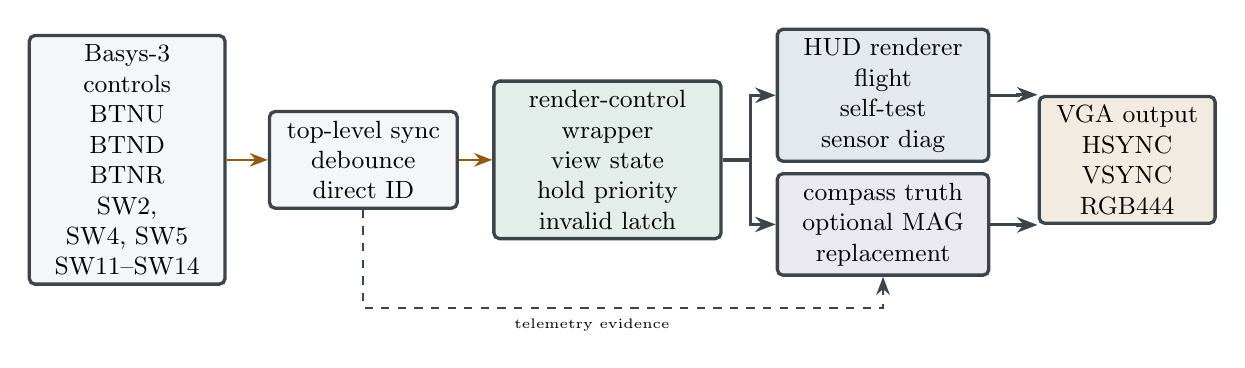
\begin{tikzpicture}[x=1cm,y=1cm]
  \node[cfBlock, text width=2.25cm] (board) at (0,0)
        {Basys-3 controls\\BTNU\\BTND\\BTNR\\SW2, SW4, SW5\\SW11--SW14};
  \node[cfBlock, text width=2.15cm] (sync) at (3.0,0)
        {top-level sync\\debounce\\direct ID};
  \node[cfBlock, text width=2.65cm, fill=cfgreen!12] (wrap) at (6.1,0)
        {render-control wrapper\\view state\\hold priority\\invalid latch};
  \node[cfBlock, text width=2.45cm, fill=cfblue!12] (hud) at (9.6,0.82)
        {HUD renderer\\flight\\self-test\\sensor diag};
  \node[cfBlock, text width=2.45cm, fill=cfpurple!12] (compass) at (9.6,-0.82)
        {compass truth\\optional MAG\\replacement};
  \node[cfBlock, text width=2.0cm, fill=cfamber!12] (vga) at (12.7,0)
        {VGA output\\HSYNC\\VSYNC\\RGB444};

  \draw[cfCtrl] (board) -- (sync);
  \draw[cfCtrl] (sync) -- (wrap);
  \draw[cfArrow] (wrap.east) -- ++(0.35,0) |- (hud.west);
  \draw[cfArrow] (wrap.east) -- ++(0.35,0) |- (compass.west);
  \draw[cfArrow] (hud.east) -- ++(0.35,0) |- (vga.north west);
  \draw[cfArrow] (compass.east) -- ++(0.35,0) |- (vga.south west);
  \draw[cfDashed] (sync.south) -- ++(0,-1.25) -| node[pos=0.22,below,font=\tiny]{telemetry evidence} (compass.south);
\end{tikzpicture}
\caption{Unified VGA render-control boundary.  Control synchronization remains
in the top level; view resolution and renderer enables are owned by the wrapper.}
\label{fig:unified-boundary}
\end{figure}

\subsection{Legal Views and Priority}

\begin{table}[H]
\centering
\caption{Unified view states.}
\label{tab:view-states}
\small
\begin{tabularx}{\linewidth}{L{0.21\linewidth} L{0.12\linewidth} L{0.20\linewidth} Y}
\toprule
\textbf{View} & \textbf{ID} & \textbf{Legal when} & \textbf{Visible behavior} \\
\midrule
\view{VIEW_FLIGHT_HUD} & \bits{3'd0} & Always & Normal flight HUD and primary telemetry visualization. \\
\view{VIEW_COMPASS_TRUTH} & \bits{3'd1} & Compass page synthesized & Optional full-screen MAG/heading diagnostic replacement page. \\
\view{VIEW_SELFTEST_HUD} & \bits{3'd2} & Always & Normal HUD renderer driven by self-test stimulus. \\
\view{VIEW_SENSOR_DIAG} & \bits{3'd3} & Always & Sensor diagnostic page when synthesized; HUD visual fallback when not synthesized. \\
\view{VIEW_SCIENCE_EXPLAIN} & \bits{3'd4} & Science pages synthesized & Compact physics/environment evidence overlay. \\
\view{VIEW_SCIENCE_WIND} & \bits{3'd5} & Science pages synthesized & Compact wind triangle and dispersion evidence overlay. \\
\view{VIEW_SCIENCE_INTEGRITY} & \bits{3'd6} & Science pages synthesized & Compact sensor-integrity correlation overlay. \\
Reserved & \bits{3'd7} & Never & Direct requests are rejected and latch \sig{cfg_invalid_view_sys}. \\
\bottomrule
\end{tabularx}
\end{table}

\begin{figure}[H]
\centering
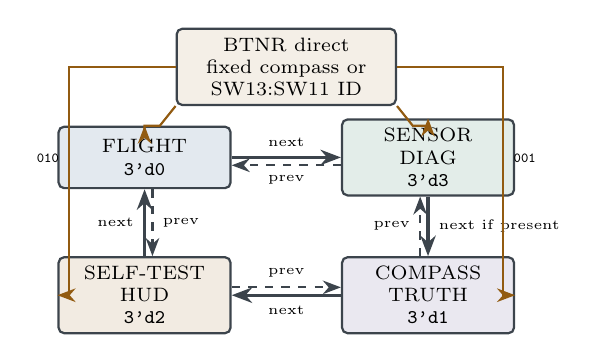
\begin{tikzpicture}[x=1cm,y=1cm]
  \node[cfState=cfblue, text width=1.95cm] (hud) at (0,0) {FLIGHT\\\bits{3'd0}};
  \node[cfState=cfgreen, text width=1.95cm] (diag) at (3.6,0) {SENSOR\\DIAG\\\bits{3'd3}};
  \node[cfState=cfpurple, text width=1.95cm] (truth) at (3.6,-1.75) {COMPASS\\TRUTH\\\bits{3'd1}};
  \node[cfState=cfamber, text width=1.95cm] (self) at (0,-1.75) {SELF-TEST\\HUD\\\bits{3'd2}};
  \node[cfSmall, text width=2.55cm, fill=cfamber!10] (direct) at (1.8,1.15)
        {BTNR direct\\fixed compass or\\SW13:SW11 ID};

  \draw[cfArrow] (hud.east) -- node[above,font=\tiny]{next} (diag.west);
  \draw[cfArrow] (diag.south) -- node[right,font=\tiny]{next if present} (truth.north);
  \draw[cfArrow] (truth.west) -- node[below,font=\tiny]{next} (self.east);
  \draw[cfArrow] (self.north) -- node[left,font=\tiny]{next} (hud.south);
  \draw[cfDashed] ([yshift=-0.10cm]diag.west) -- node[below,font=\tiny]{prev} ([yshift=-0.10cm]hud.east);
  \draw[cfDashed] ([xshift=-0.10cm]truth.north) -- node[left,font=\tiny]{prev} ([xshift=-0.10cm]diag.south);
  \draw[cfDashed] ([yshift=0.10cm]self.east) -- node[above,font=\tiny]{prev} ([yshift=0.10cm]truth.west);
  \draw[cfDashed] ([xshift=0.10cm]hud.south) -- node[right,font=\tiny]{prev} ([xshift=0.10cm]self.north);
  \draw[cfCtrl] (direct.south west) -- ++(-0.2,-0.25) -| (hud.north);
  \draw[cfCtrl] (direct.south east) -- ++(0.2,-0.25) -| (diag.north);
  \draw[cfCtrl] (direct.east) -- ++(1.35,0) |- node[pos=0.20,right,font=\tiny]{\bits{001}} (truth.east);
  \draw[cfCtrl] (direct.west) -- ++(-1.35,0) |- node[pos=0.20,left,font=\tiny]{\bits{010}} (self.west);
\end{tikzpicture}
\caption{Registered view navigation.  Direct valid requests have priority over
next/previous pulses.  Reserved direct IDs and disabled compass requests do not
change \sig{view_sel_sys}.}
\label{fig:view-state}
\end{figure}

The effective-view priority is:
\[
V_{\mathrm{effective}} =
\begin{cases}
\view{VIEW_COMPASS_TRUTH}, & \text{if compass hold is asserted and compass page is present},\\
\view{VIEW_SELFTEST_HUD},  & \text{if self-test hold is asserted},\\
V_{\mathrm{registered}},  & \text{otherwise.}
\end{cases}
\]

\subsection{Active Interface Contract}

\begin{longtable}{L{0.25\linewidth} L{0.16\linewidth} L{0.50\linewidth}}
\caption{Unified interface contract.}
\label{tab:interface}\\
\toprule
\textbf{Interface group} & \textbf{Width/domain} & \textbf{Contract} \\
\midrule
\endfirsthead
\toprule
\textbf{Interface group} & \textbf{Width/domain} & \textbf{Contract} \\
\midrule
\endhead
View-control pulses &
1-bit SYS &
\sig{view_next_pulse_sys}, \sig{view_prev_pulse_sys}, and
\sig{view_direct_valid_sys} are one-cycle, synchronized pulses produced above
the wrapper. \\
Direct view ID &
3-bit SYS &
\sig{view_direct_id_sys[2:0]} is either fixed to compass truth by the top level
or loaded from synchronized \sig{SW13:SW11} when
\param{USE_SWITCH_ENCODED_VIEW_SELECT != 0} and SW3 MAG1 bench mode plus SW2+SW6
diagnostic fault injection are inactive.  During either SW11--SW13 ownership
mode the top-level arbiter emits reserved ID \bits{3'b111} so the wrapper
rejects the request and holds \sig{view_sel_sys}. \\
Legacy holds &
1-bit SYS levels &
\sig{legacy_compass_page_hold_sys} and \sig{legacy_selftest_hold_sys} preserve
button/switch hold behavior without coupling compass replacement to self-test
stimulus. \\
Render-state outputs &
3-bit and 1-bit SYS &
\sig{view_sel_sys}, \sig{view_effective_sys}, \sig{view_changed_pulse_sys}, and
\sig{cfg_invalid_view_sys} are deterministic observability points. \\
Telemetry payloads &
48-bit payloads, 32-bit timestamps, 16-bit sequences/ages, 8-bit statuses &
Sensor, derived, extension, navigation, wind, authority, safety, I2C, build,
and schema fields are passed through with original widths. \\
Pixel interface &
PIX clock/reset plus RGB444 &
\sig{pix_clk} and \sig{pix_rst} clock the renderers.  The board-facing output
is \sig{vga_hsync}, \sig{vga_vsync}, and \sig{vga_rgb[11:0]}. \\
\bottomrule
\end{longtable}

\section{Rendering, Telemetry, and Timing}

The unified wrapper does not reinterpret telemetry.  Raw sensor evidence,
derived estimator values, extension-hub fields, rendered pixels, and diagnostic
representations remain separate.  Invalid or stale telemetry is represented by
status colors, warning fields, or diagnostic page annotations rather than by
silently dropping data.

\begin{figure}[H]
\centering
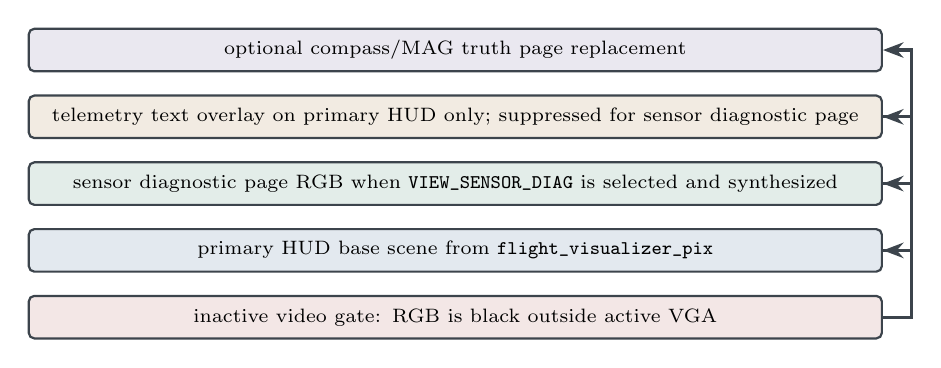
\begin{tikzpicture}[node distance=0.28cm]
  \node[cfLayer=cfred] (black) {inactive video gate: RGB is black outside active VGA};
  \node[cfLayer=cfblue, above=of black] (base) {primary HUD base scene from \file{flight_visualizer_pix}};
  \node[cfLayer=cfgreen, above=of base] (diag) {sensor diagnostic page RGB when \sig{VIEW_SENSOR_DIAG} is selected and synthesized};
  \node[cfLayer=cfamber, above=of diag] (text) {telemetry text overlay on primary HUD only; suppressed for sensor diagnostic page};
  \node[cfLayer=cfpurple, above=of text] (truth) {optional compass/MAG truth page replacement};
  \draw[cfArrow] (black.east) -- ++(0.36,0) |- (base.east);
  \draw[cfArrow] (base.east) -- ++(0.36,0) |- (diag.east);
  \draw[cfArrow] (diag.east) -- ++(0.36,0) |- (text.east);
  \draw[cfArrow] (text.east) -- ++(0.36,0) |- (truth.east);
\end{tikzpicture}
\caption{Deterministic compositor and replacement priority.}
\label{fig:layer-stack}
\end{figure}

\begin{figure}[H]
\centering
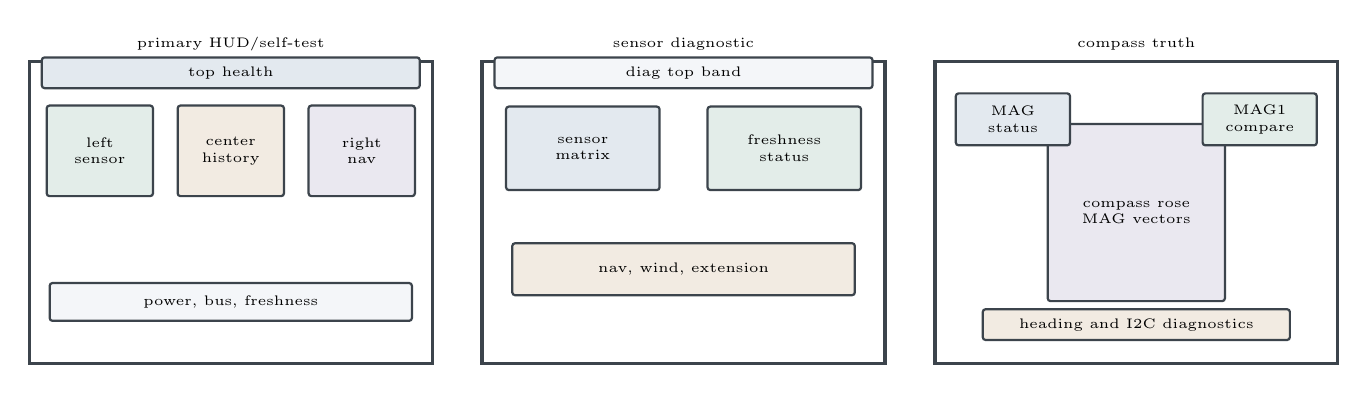
\begin{tikzpicture}[x=0.008cm,y=-0.008cm]
  \draw[screen] (0,0) rectangle (640,480);
  \node[font=\tiny] at (320,-28) {primary HUD/self-test};
  \node[screenRect, fill=cfblue!12] at (320,18) [minimum width=4.8cm, minimum height=0.26cm] {top health};
  \node[screenRect, fill=cfgreen!12] at (112,142) [minimum width=1.35cm, minimum height=1.15cm] {left\\sensor};
  \node[screenRect, fill=cfamber!12] at (320,142) [minimum width=1.35cm, minimum height=1.15cm] {center\\history};
  \node[screenRect, fill=cfpurple!12] at (528,142) [minimum width=1.35cm, minimum height=1.15cm] {right\\nav};
  \node[screenRect, fill=cfgray] at (320,382) [minimum width=4.6cm, minimum height=0.48cm] {power, bus, freshness};

  \begin{scope}[xshift=5.75cm]
    \draw[screen] (0,0) rectangle (640,480);
    \node[font=\tiny] at (320,-28) {sensor diagnostic};
    \node[screenRect, fill=cfgray] at (320,18) [minimum width=4.8cm, minimum height=0.26cm] {diag top band};
    \node[screenRect, fill=cfblue!12] at (160,138) [minimum width=1.95cm, minimum height=1.06cm] {sensor\\matrix};
    \node[screenRect, fill=cfgreen!12] at (480,138) [minimum width=1.95cm, minimum height=1.06cm] {freshness\\status};
    \node[screenRect, fill=cfamber!12] at (320,330) [minimum width=4.35cm, minimum height=0.66cm] {nav, wind, extension};
  \end{scope}

  \begin{scope}[xshift=11.50cm]
    \draw[screen] (0,0) rectangle (640,480);
    \node[font=\tiny] at (320,-28) {compass truth};
    \node[screenRect, fill=cfpurple!12] at (320,240) [minimum width=2.25cm, minimum height=2.25cm] {compass rose\\MAG vectors};
    \node[screenRect, fill=cfblue!12] at (124,92) [minimum width=1.45cm, minimum height=0.66cm] {MAG\\status};
    \node[screenRect, fill=cfgreen!12] at (516,92) [minimum width=1.45cm, minimum height=0.66cm] {MAG1\\compare};
    \node[screenRect, fill=cfamber!12] at (320,418) [minimum width=3.9cm, minimum height=0.38cm] {heading and I2C diagnostics};
  \end{scope}
\end{tikzpicture}
\caption{Preserved and extended layout diagrams: primary HUD/self-test, sensor
diagnostic page, and optional compass truth page.}
\label{fig:layouts}
\end{figure}

\begin{figure}[H]
\centering
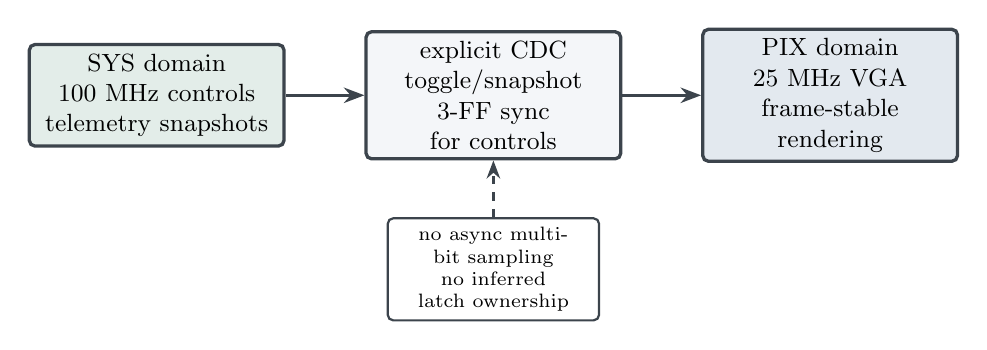
\begin{tikzpicture}[node distance=0.82cm and 1.0cm]
  \node[cfBlock, fill=cfgreen!12] (sys) {SYS domain\\100 MHz controls\\telemetry snapshots};
  \node[cfBlock, right=of sys, fill=cfgray] (cdc) {explicit CDC\\toggle/snapshot\\3-FF sync for controls};
  \node[cfBlock, right=of cdc, fill=cfblue!12] (pix) {PIX domain\\25 MHz VGA\\frame-stable rendering};
  \node[cfSmall, below=0.72cm of cdc] (rule) {no async multi-bit sampling\\no inferred latch ownership};
  \draw[cfArrow] (sys) -- (cdc);
  \draw[cfArrow] (cdc) -- (pix);
  \draw[cfDashed] (rule.north) -- (cdc.south);
\end{tikzpicture}
\caption{Clock and timing contract preserved by the unified boundary.}
\label{fig:cdc-contract}
\end{figure}

\section{Resolved Conflicts}

\begin{longtable}{L{0.25\linewidth} L{0.31\linewidth} L{0.34\linewidth}}
\caption{Conflicting assumptions and final decisions.}
\label{tab:conflicts}\\
\toprule
\textbf{Conflict} & \textbf{Observed assumption} & \textbf{Unified decision} \\
\midrule
\endfirsthead
\toprule
\textbf{Conflict} & \textbf{Observed assumption} & \textbf{Unified decision} \\
\midrule
\endhead
Sensor diagnostic default &
Some drafts describe \param{USE_SENSOR_DIAG_PAGE=0} as the default.  The live
top-level sets \param{USE_SENSOR_DIAG_PAGE=1}. &
Document the live source-default as enabled.  Preserve legal fallback behavior
for builds that set the parameter to 0. \\
Compass page default ownership &
The child compass page has its own \param{COMPASS_TRUTH_PAGE_DEFAULT}
parameter. &
Wrapper owns default-view policy.  The child instance receives
\param{COMPASS_TRUTH_PAGE_DEFAULT(0)} so it cannot override the HUD stream. \\
BTNR behavior &
Older drafts treat BTNR as fixed direct compass select.  The live top supports
switch-encoded direct ID selection. &
Preserve both contracts: active default uses SW13:SW11 encoded IDs only outside
MAG1 bench mode and SW2+SW6 diagnostic fault injection; setting
\param{USE_SWITCH_ENCODED_VIEW_SELECT=0} restores fixed compass request. \\
Self-test versus compass hold &
Earlier top-level wiring risked coupling one control to both HUD self-test data
and the full-screen compass page. &
Separate \sig{legacy_selftest_hold_sys} from
\sig{legacy_compass_page_hold_sys}.  Compass hold masks self-test only when the
truth page is synthesized. \\
Invalid direct ID handling &
Reserved encodings could be interpreted as don't-care in a loose UI spec. &
Reserved IDs are explicit errors: preserve \sig{view_sel_sys}, assert
\sig{cfg_invalid_view_sys}, and clear only through
\sig{cfg_invalid_view_clear_sys} or reset. \\
Frame stability &
Textual drafts discuss frame-stable behavior at different levels of detail. &
Use existing renderer CDC and page-select synchronization.  Do not sample raw
human inputs or multi-bit telemetry directly in the PIX domain. \\
\bottomrule
\end{longtable}

\section{Completed Final RTL Module}

The final implementation is the live RTL module below.  The listing is included
from the project source file so this report stays aligned with the implementation
used by \file{caelumfusion_top_vga.v}.

\lstinputlisting[
  caption={Final unified RTL module: \file{caelumfusion_vga_render_control.v}},
  label={lst:final-rtl}
]{../CaelumFusion_Flight_Control_System.srcs/sources_1/new/caelumfusion_vga_render_control.v}

\section{Migration Notes}

\begin{enumerate}
  \item Replace separate top-level view-selection glue, direct page enables, and
        duplicated HUD/compass routing with one
        \file{caelumfusion_vga_render_control} instance.
  \item Keep raw board controls at the top-level boundary.  Synchronize and
        debounce BTNU, BTND, BTNR, and switch levels before driving the wrapper.
  \item Drive \sig{view_next_pulse_sys} from BTNU, \sig{view_prev_pulse_sys}
        from BTND, and \sig{view_direct_valid_sys} from BTNR.  In the active
        encoded-selector build, pass BTNR and SW13:SW11 through
        \file{caelumfusion_vga_direct_view_arbiter_sys}; the arbiter drives
        \sig{view_direct_id_sys} from \{\sig{SW13}, \sig{SW12}, \sig{SW11}\}
        only while SW3 MAG1 bench mode and SW2+SW6 diagnostic fault injection
        are inactive, and otherwise drives reserved \bits{3'b111}.  If encoded
        selection is disabled, drive \view{VIEW_COMPASS_TRUTH}.
  \item Preserve \sig{legacy_selftest_hold_sys = sw_selftest_level_sys}
        except where diagnostic fault injection intentionally masks self-test.
        Preserve \sig{legacy_compass_page_hold_sys = SW4 | SW14}.
  \item Bind \param{ENABLE_SENSOR_DIAG_PAGE} to
        \param{USE_SENSOR_DIAG_PAGE}.  A value of 0 must keep
        \view{VIEW_SENSOR_DIAG} legal but visually fall back to primary HUD RGB.
  \item Bind \param{ENABLE_COMPASS_TRUTH_PAGE} to
        \param{USE_COMPASS_TRUTH_PAGE}.  A value of 0 must make direct compass
        requests illegal and must ignore compass hold levels.
  \item Bind \param{ENABLE_SCIENCE_PAGES} to \param{USE_SCIENCE_PAGES}.  A
        value of 0 must make direct science-page IDs illegal while preserving
        the legacy HUD, diagnostic, compass, and self-test views.
  \item Leave \sig{cfg_invalid_view_clear_sys} tied low only if the board has no
        clear command.  Future debug builds should expose clear control or show
        \sig{cfg_invalid_view_sys} on LEDs, UART, or a small HUD field.
  \item Keep XDC false paths scoped from asynchronous button/switch ports to the
        first synchronizer flop only.  Do not false-path synchronized
        SYS-domain logic.
  \item Preserve the existing testbench
        \file{tb_caelumfusion_render_control_switch_encoded.v}; it is the
        focused regression for encoded direct selection, disabled compass
        rejection, reserved-ID rejection, and hold priority.
  \item Retire the older draft PDFs as design references once this unified
        source and generated PDF are reviewed.  Keep the broader system report
        only for whole-system requirements, hardware instrumentation, and
        evidence-chain context.
\end{enumerate}

\section{Verification Plan}

\begin{longtable}{L{0.27\linewidth} L{0.56\linewidth} L{0.10\linewidth}}
\caption{Recommended verification gates after migration.}
\label{tab:verification}\\
\toprule
\textbf{Gate} & \textbf{Expected evidence} & \textbf{Status} \\
\midrule
\endfirsthead
\toprule
\textbf{Gate} & \textbf{Expected evidence} & \textbf{Status} \\
\midrule
\endhead
Static RTL review &
No multiple drivers, inferred latches, unsized truncation, or async multi-bit
sampling across the wrapper interface. &
Required \\
Focused render-control simulation &
\file{tb_caelumfusion_render_control_switch_encoded.v} prints an explicit
PASS line. &
Required \\
Top-level elaboration &
\file{caelumfusion_top_vga} elaborates with the wrapper, HUD renderer, compass
page dependency, and \file{landing_nav_wind_observer}. &
Required \\
Optional build matrix &
Synthesize default, compass-enabled, sensor-diag-disabled, and text-disabled
profiles.  Record utilization and timing deltas. &
Recommended \\
Display evidence &
Capture reset HUD, self-test HUD, sensor diagnostic view, compass truth view
when enabled, invalid/stale telemetry colors, and inactive-video black level. &
Recommended \\
Documentation QA &
Compile this document and inspect the diagram pages for overlap, clipped text,
and broken listings. &
Required \\
\bottomrule
\end{longtable}

\section{Recommended Next Development Steps}

\begin{enumerate}
  \item Route \sig{view_effective_sys} and \sig{cfg_invalid_view_sys} to a small
        visible debug field, LEDs, or UART-visible status word.
  \item Add a pixel-level regression that checks sensor-diagnostic fallback when
        \param{USE_SENSOR_DIAG_PAGE=0} and text-overlay suppression when
        \param{USE_SENSOR_DIAG_PAGE=1}.
  \item Run and archive the switch-encoded render-control testbench after every
        control-map change.
  \item Build a recorded variant matrix for
        \param{USE_COMPASS_TRUTH_PAGE}, \param{USE_SENSOR_DIAG_PAGE}, and
        \param{USE_TELEMETRY_TEXT_OVERLAY}; record utilization, WNS/WHS, DRC,
        and bitstream hashes.
  \item Keep the runtime control map synchronized with the SW11--SW13
        arbitration rule: clean direct navigation requires SW3 low and either
        SW2 or SW6 low before pressing BTNR; bench and fault switches can be
        restored after the view is selected.
\end{enumerate}

\end{document}
